\chapter{\label{sec:transientes} Experimento II - Transientes}

%----------------------------------
%-------OBJETIVOS------------------
%----------------------------------
\subsection{Objetivos}
Entender o papel ...
\subsection{Introdu��o}
Introduction goes here...
\subsubsection{Diodo demodulador ou detector}
% \begin{wrapfigure}{r}{0.5\textwidth}
%  \vspace{-20pt}
%  \begin{center}
%    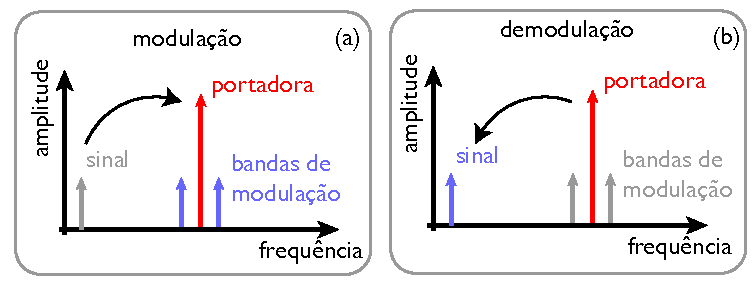
\includegraphics[width=0.5\textwidth]{mod_e_demod}
%  \end{center}
%   \vspace{-20pt}
%  \caption{Princ�pio de modula��o de demodula��o de um sinal.}
%\end{wrapfigure}
%----------------------------------
%-------PREPARA��O-----------------
%----------------------------------
\subsection{Prepara��o}
\begin{enumerate}
\item Calcule a fun��o... 
\end{enumerate}
%----------------------------------
%-------MATERIAL-----------------
%----------------------------------

%----------------------------------
%----------Roteiro-----------------
%----------------------------------
\subsection{Roteiro A - Circuito RC}
\subsubsection*{Material}
\begin{itemize}
\item Diodo de  sil�cio.
\end{itemize}
\subsubsection*{Caracteriza��o do circuito LC}
\subsection{Roteiro B - Circuito RLC}
\subsubsection*{Caracteriza��o da curva IV do diodo}
%----------------------------------
%----------Relatorio-----------------
%----------------------------------
\subsection{Relat�rio}

